{\color{indiagreen}\subsection{Plinski zakoni}}
\begin{align*}
	n &= konst. \text{množina snovi je konstantna}\\
	\frac{pV}{T} &= nR = konst.\\
	{\color{bostonuniversityred}\frac{p_1V_1}{T_1}} &= {\color{bostonuniversityred}\frac{p_2V_2}{T_2}} \text{Splošna plinska enačba za konstantno množino snovi}\\
\end{align*}
\begin{enumerate}
	\item T = konst in n = konst $\rightarrow$ \textbf{Izotermna sprememba}\\
		\begin{align*}
			{\color{bostonuniversityred}p_1V_1} &= {\color{bostonuniversityred}p_2V_2}\text{Boylov zakon}\\
			p_1 &= \frac{p_2V_2}{V_1}\\
		\end{align*}
		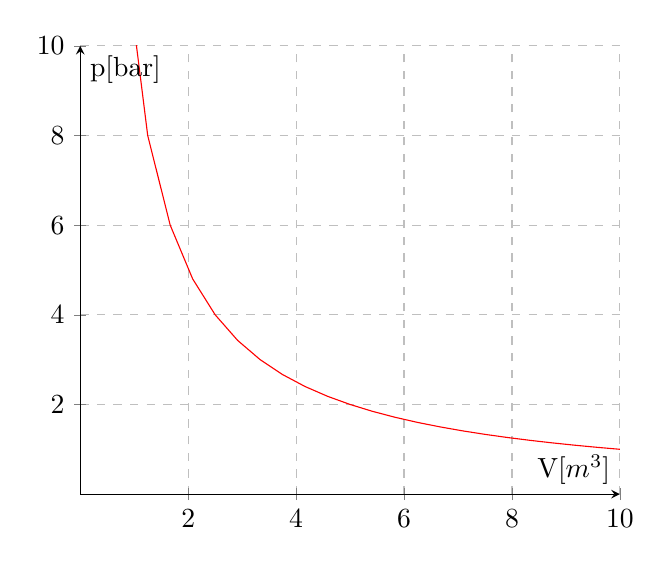
\begin{tikzpicture}
			\begin{axis}[
			    xlabel={V[$m^3$]},
			    ylabel={p[bar]},
			    xmin=0, xmax=10,
			    ymin=0, ymax=10,
			    xtick={0,2,4,6,8,10},
			    ytick={0,2,4,6,8,10},
			    ymajorgrids=true,
			    xmajorgrids=true,
			    grid style=dashed,
			    axis lines=middle,
			]
			\addplot[domain=0:10,red] {10/x};
			\end{axis}
		\end{tikzpicture}
	\item V = konst in n = konst $\rightarrow$ \textbf{Izohorna sprememba}\\
		\begin{align*}
			{\color{bostonuniversityred}\frac{p_1}{T_1}} &= {\color{bostonuniversityred}\frac{p_2}{T_2}} \text{Amontonsov zakon}\\
			p_1 &= T_1\frac{p_2}{T_2}\\
		\end{align*}
		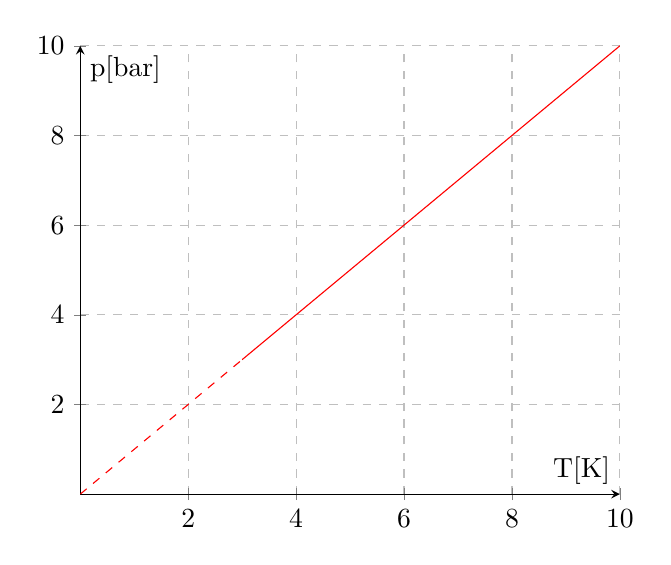
\begin{tikzpicture}
			\begin{axis}[
			    xlabel={T[K]},
			    ylabel={p[bar]},
			    xmin=0, xmax=10,
			    ymin=0, ymax=10,
			    xtick={0,2,4,6,8,10},
			    ytick={0,2,4,6,8,10},
			    ymajorgrids=true,
			    xmajorgrids=true,
			    grid style=dashed,
			    axis lines=middle,
			]
			\addplot[domain=0:3,red, dashed] {x};
			\addplot[domain=3:10,red] {x};
			\end{axis}
		\end{tikzpicture}\\
		*Pri crtkani crti postane kapljevina\\
	\item p = konst in n = konst $\rightarrow$ \textbf{Izobarna sprememba}\\
		\begin{align*}
			{\color{bostonuniversityred}\frac{V_1}{T_1}} &= {\color{bostonuniversityred}\frac{V_2}{T_2}} \text{Amontonsov zakon}\\
			V_1 &= T_1\frac{V_2}{T_2}\\
		\end{align*}
		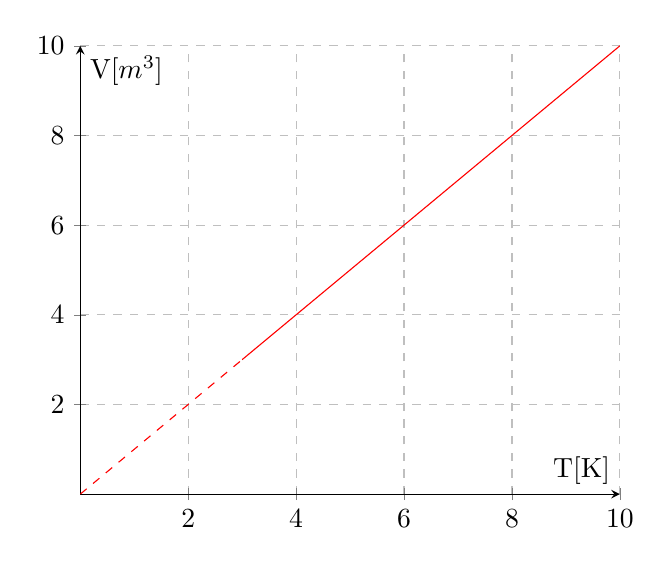
\begin{tikzpicture}
			\begin{axis}[
			    xlabel={T[K]},
			    ylabel={V[$m^3$]},
			    xmin=0, xmax=10,
			    ymin=0, ymax=10,
			    xtick={0,2,4,6,8,10},
			    ytick={0,2,4,6,8,10},
			    ymajorgrids=true,
			    xmajorgrids=true,
			    grid style=dashed,
			    axis lines=middle,
			]
			\addplot[domain=0:3,red, dashed] {x};
			\addplot[domain=3:10,red] {x};
			\end{axis}
		\end{tikzpicture}\\
		*Pri crtkani crti postane kapljevina\\
\end{enumerate}